\documentclass{beamer}
\mode<presentation>
{
\usepackage{dis-template}
}
\usepackage{listings}
\usepackage{hyperref}
\usepackage{textcomp}
\usepackage{soul}
\usepackage{color}
\definecolor{comments}{HTML}{50c878}
\lstset{language=C++,
  basicstyle=\ttfamily,
  keywordstyle=\color{blue}\ttfamily,
  stringstyle=\color{red}\ttfamily,
  commentstyle=\color{comments}\ttfamily,
  breaklines=true
}
\graphicspath{{slides/}} % TODO: eliminate this hack, necessary because scons builds at repository root

%---------------------------------------------------------------------
\titlepageinit{4}{Power Systems}{11 \& 12 Feb 2015 (Week 4)}
%---------------------------------------------------------------------
\begin{document}
%---------------------------------------------------------------------
\begin{frame}
\titlepage

\setcounter{tocdepth}{1}
\tableofcontents
\end{frame}

% LAB PREPARATION
% Setup capacitor frequency demo with:
% Ceramic capacitor, 100ohm 0.1uF
% Aluminum capacitor, 1ohm 10uF
% Set up SMPS demo

%---------------------------------------------------------------------
\section{SMPS Recap} % [?? mins]
%---------------------------------------------------------------------
\begin{frame}
\centering \huge Switching Power Supply Recap
\end{frame}

%---------------------------------------------------------------------
\subsection{Boost Converter Theory}

\begin{frame}
\frametitle{Boost Converter Circuit}
\begin{columns}[t]
\column{0.646\textwidth}
\begin{itemize}
  \item DC-to-DC switching power supply generating output voltage higher than input
  \item Uses inductor as storage element
  \item Efficient, no losses in ideal case
  \begin{itemize}
    \item Non-idealities: wire resistance, diode and transistor losses
  \end{itemize}
  \item Capacitive filter to smooth output voltage
\end{itemize}

\column{0.323\textwidth}
\begin{figure}
  \centering
  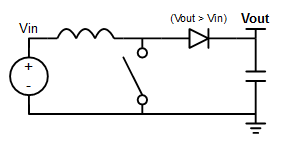
\includegraphics[scale=0.33]{images-dis4/smps-boost} \\
  Boost Converter
\end{figure}
\end{columns}
\end{frame}

\begin{frame}
\frametitle{Boost Converter Operation}
\begin{columns}[t]
\column{0.646\textwidth}
\begin{itemize}
  \item Inductor charges when switch is closed
  \begin{itemize}
    \item Energy stored in inductor by magnetic field, current through inductor increases
    \item Diode prevents higher output voltage from flowing back to source
  \end{itemize}
  \item<2-> Inductor dischanges when switch is open
  \begin{itemize}
    \item Magnetic field dissipates, current through inductor decreases
    \item Inductor voltage polarity reversed, generating voltage over input
    \item Current flows through diode, output capacitor charged
  \end{itemize}  
\end{itemize}

\column{0.323\textwidth}
\begin{figure}
  \centering
  \only<1>{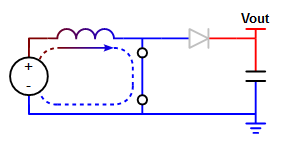
\includegraphics[scale=0.33]{images-dis4/smps-boost-closed} \\
  Switch Closed}
  \only<2>{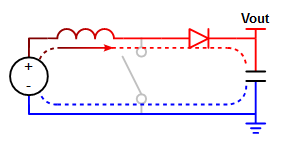
\includegraphics[scale=0.33]{images-dis4/smps-boost-open} \\
  Switch Open}
\end{figure}
\end{columns}
\end{frame}

\begin{frame}
\frametitle{Boost Converter Control}
\begin{columns}[t]
\column{0.646\textwidth}
\begin{itemize}
  \item If switch cycled fast enough, inductor does not fully discharge
  \item Can do a lot of math, but output voltage is function of duty cycle $D$
  \begin{itemize}
    \item $V_{out}=\frac{1}{1-D} V_{in}$
  \end{itemize}
\end{itemize}

\column{0.323\textwidth}
\begin{figure}
  \centering
  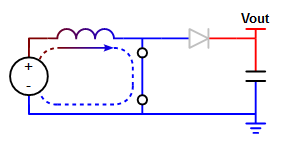
\includegraphics[scale=0.33]{images-dis4/smps-boost-closed} \\
  Inductor charging \\
  \hfill \\
  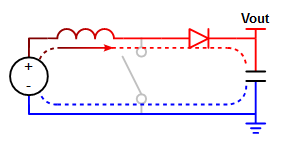
\includegraphics[scale=0.33]{images-dis4/smps-boost-open} \\
  Inductor discharging
\end{figure}
\end{columns}
\end{frame}

\begin{frame}
\frametitle{Check your Understanding {\small (Live Demo Edition!)}}
\begin{columns}[t]
\column{0.646\textwidth}
\begin{itemize}
  \item So I've got a boost converter set up...
  \begin{itemize}
    \item One probe on the switch
    \item Another probe on the output
  \end{itemize}
  \item It's running at steady-state
  \item<2-> Which scope waveform is the switch?
  \item<3-> Is the output waveform what you expect?
  \item<4-> On the switch waveform...
  \begin{itemize}
    \item<4-> Which part is the switch closed? 
    \item<5-> Which part is the switch opened?
  \end{itemize}
\end{itemize}

\column{0.323\textwidth}
\begin{figure}
  \centering
  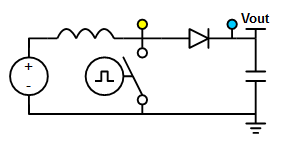
\includegraphics[scale=0.33]{images-dis4/smps-boost-probed} \\
  Boost Circuit
\end{figure}
\end{columns}
\end{frame}

\begin{frame}
\frametitle{Check your Understanding {\small (Live Demo Edition!)}}
\begin{columns}[t]
\column{0.646\textwidth}
\begin{itemize}
  \item So I've got a boost converter set up...
  \begin{itemize}
    \item One probe on the switch
    \item Another probe on the output
  \end{itemize}
  \item A magic chip regulates the output to 12v
  \begin{itemize}
    \item Duty cycle is adjusted to maintain voltage
    \item Remember: $V_{out}=\frac{1}{1-D} V_{in}$
  \end{itemize}
  \item What happens if I...
  \begin{itemize}
    \item <2->Increase the input voltage?
    \begin{itemize}
      \item <3->Duty cycle decreases, current decreases
    \end{itemize}
    \item <4->Decrease the input voltage?
    \begin{itemize}
      \item <5->Duty cycle increases, current increases
    \end{itemize}
  \end{itemize}
\end{itemize}

\column{0.323\textwidth}
\begin{figure}
  \centering
  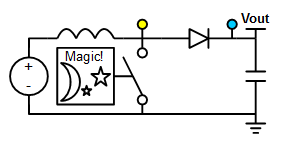
\includegraphics[scale=0.33]{images-dis4/smps-boost-probed-magic} \\
  Boost Circuit
\end{figure}
\end{columns}
\end{frame}

%---------------------------------------------------------------------
\subsection{Related Topologies}

\begin{frame}
\frametitle{Buck Converter Circuit \small{(for your reference)}}
\begin{columns}[t]
\column{0.646\textwidth}
\begin{itemize}
  \item DC-to-DC switching power supply generating output voltage \textit{lower} than input
  \item Similar principle to boost converter
  \begin{itemize}
    \item $V_{out}=D V_{in}$
  \end{itemize}
  \hfill \\
  \item Also exists buck-boost converters, where output can be greater than, equal to, or less than the input
\end{itemize}

\column{0.323\textwidth}
\begin{figure}
  \centering
  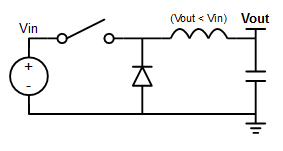
\includegraphics[scale=0.33]{images-dis4/smps-buck} \\
  Buck Converter
\end{figure}
\end{columns}
\end{frame}

\begin{frame}
\frametitle{Questions?}
\centering
{\huge got it?} \\
\vspace{20px}
\tiny{power supply pros, right?}
\end{frame}

%---------------------------------------------------------------------
\section{Practical Application} % [?? mins]
%---------------------------------------------------------------------
\begin{frame}
\centering \huge Practical Application
\end{frame}

%---------------------------------------------------------------------
\subsection{Basics}

\begin{frame}
\frametitle{Automatic Feedback Control}
\begin{columns}[t]
\column{0.646\textwidth}
\begin{itemize}
  \item So, what is the switch-controlling magic?
  \item Feedback control: chip has logic to regulate the voltage on the feedback pin to an internal 1.245v reference
  \item Pop quiz: what resistor divider do I use to regulate the output to 7.2v?
  \begin{itemize}
    \item Use 8.2k$\Omega$ for the lower resistor
    \item<2-> ... and 39k$\Omega$ For the higher resistor
    \item<2-> Why these numbers? Preferred numbers!
  \end{itemize}
\end{itemize}

\column{0.323\textwidth}
\begin{figure}
  \centering
  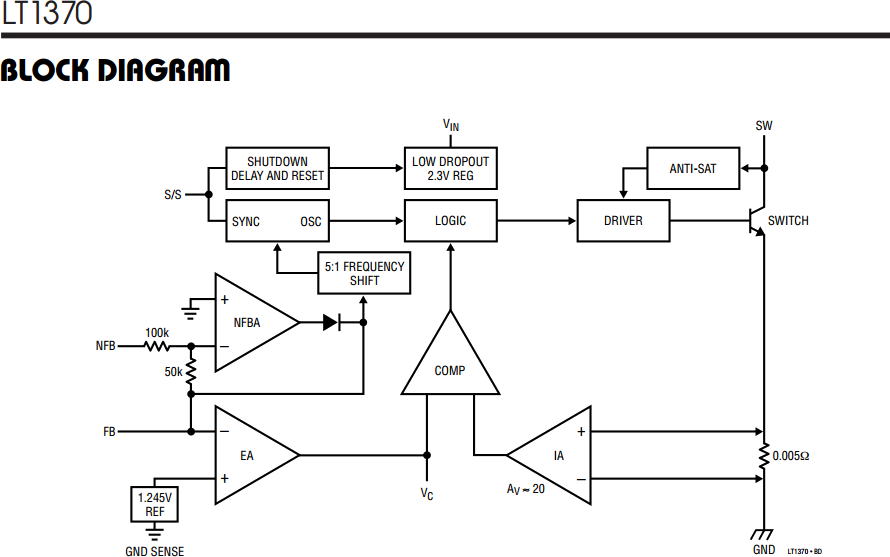
\includegraphics[width=1.0\columnwidth]{images-dis4/lt1370-block} \\
  LT1370 Block Diagram \\
  \hfill \\
  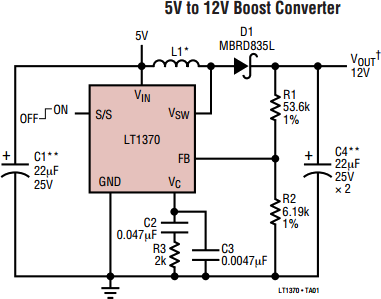
\includegraphics[width=0.66\columnwidth]{images-dis4/lt1370-application} \\
  Application circuit \\
  \tiny{source: datasheet, Linear Technology}
\end{figure}
\end{columns}
\end{frame}

%---------------------------------------------------------------------
\subsection{Issues}

\begin{frame}
\frametitle{Noise {\small (Live Demo Edition!)}}
\begin{columns}[t]
\column{0.646\textwidth}
\begin{itemize}
  \item Let's take a closer look at the output
  \begin{itemize}
    \item Specifically, note the ripple near the switch toggling
  \end{itemize}
  \item What issues might this cause?
  \item What do you think are some ways to reduce noise?
\end{itemize}

\column{0.323\textwidth}
\begin{figure}
  \centering
  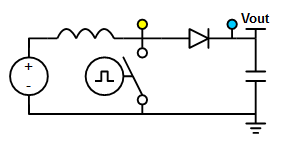
\includegraphics[scale=0.33]{images-dis4/smps-boost-probed} \\
  Boost Circuit
\end{figure}
\end{columns}
\end{frame}

\begin{frame}
\frametitle{Capacitors at High Frequencies {\small (Live Demo Edition!)}}
\begin{columns}[t]
\column{0.646\textwidth}
\begin{itemize}
  \item Output smoothing is critical for proper operation, depends on output capacitors
  \item Not all capacitors are created equal
  \begin{itemize}
    \item Ceramic, tantalum, aluminum, ...
  \end{itemize}
  \item Live demo
  \begin{itemize}
    \item Expect both filters to behave the same: \\
    $Gain=\frac{1}{\sqrt{1+(\omega R C)^2}}$, $\phi=atan(-\omega R C)$ \\
    (gain and phase dependent on only RC) \\
    \item <2-> As frequency increases, behavior diverges
    \item <2-> Capacitors become inductive - no longer a good filter
  \end{itemize}
\end{itemize}

\column{0.323\textwidth}
\begin{figure}
  \centering
  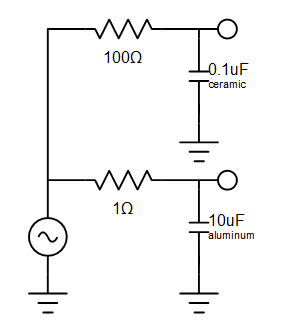
\includegraphics[scale=0.33]{images-dis4/rc-demo} \\
  RC filter demo circuit
\end{figure}
\end{columns}
\end{frame}

\begin{frame}
\frametitle{Layout Guidelines}
\begin{columns}[t]
\column{0.646\textwidth}
\begin{itemize}
  \item Switching power supplies are layout sensitive
  \begin{itemize}
    \item Part placement and routing matters!
  \end{itemize}
  \item Tips from the datasheet:
  \begin{itemize}
    \item Keep output diode, switch pin, output capacitor as short as possible
    \item Minimize length and area of switch pin
    \item Minimize high frequency current path (switch, diode, capacitor)
  \end{itemize}
  \item Read the datasheet!
\end{itemize}

\column{0.323\textwidth}
\begin{figure}
  \centering
  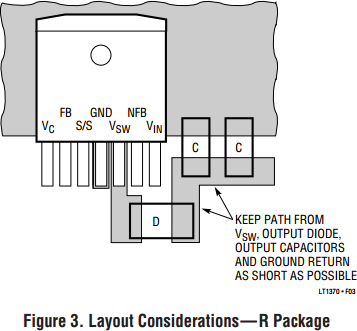
\includegraphics[width=1.0\columnwidth]{images-dis4/lt1370-layout} \\
  Recommended layout \\
  \tiny (uses surface-mount components) \\
  \tiny source: datasheet, Linear Technology
\end{figure}
\end{columns}
\end{frame}

%---------------------------------------------------------------------
\section{Summary} % [?? mins]

\begin{frame}
\frametitle{Summary}
Summary
\begin{itemize}
  \item Boost converters step up a DC voltage to a higher DC voltage
  \item LT1370 uses feedback control to do voltage regulation
  \item Follow recommended layout guidelines during PCB design
\end{itemize}
Parts Handout
\begin{itemize}
  \item Get a battery and charger!
  \begin{itemize}
    \item Please, keep explosions and flames to a minimum
  \end{itemize}
\end{itemize}
Office hours for the rest of the section
\begin{itemize}
  \item PCB deadline coming up in a week! Need help? Get it now!
  \item Need tips on mechanical fabrication? Get some here!
\end{itemize}
\end{frame}

\end{document}
